\begin{name}
	{\tenchude}
	{\tendethi}
	{\tentruong}
	{\thoigian}
\end{name}
\TN
\Opensolutionfile{ans}[ans/11-CK1-Toan-tu-tam-De-2-Phan-1]
%=======Câu 1
\begin{ex}%[1D1N4-2]
	Tập xác định của hàm số  $y=\sin x$ là
	\choice
	{\True $\mathbb{R}$}
	{$[-1;1]$}
	{$\mathbb{R}\setminus \{-1;1\}$}
	{$(-1;1)$}
	\loigiai{	Tập xác định của hàm số  $y=\sin x$ là $\mathscr{D}=\mathbb{R}$.}
\end{ex}

%=======Câu 2
\begin{ex}%[1D1N5-3]
	Tập nghiệm của phương trình $\cos x=0$ là
	\choice
	{$\mathbb{R}$}
	{\True $\left\{ \dfrac{\pi}{2}+k\pi |k \in \mathbb{Z}\right\}$}
	{$\left\{ \dfrac{\pi}{2}+k2\pi |k \in \mathbb{Z}\right\}$}
	{$\left\{k\pi |k \in \mathbb{Z}\right\}$}
	\loigiai{Ta có $\cos x=0\Leftrightarrow  \dfrac{\pi}{2}+k\pi , \,(k \in \mathbb{Z})$ .}
\end{ex}

%=======Câu 3
\begin{ex}%[1D2N2-4]
	Cho cấp số cộng \( \left(u_n\right) \), biết \( u_1 = 3 \) và \( u_2 = 6 \). Tìm số hạng thứ $8$ của cấp số cộng trên.
	\choice
	{$15$}
	{$21$}
	{$27$}
	{\True $24$}
	\loigiai{Ta có công sai của cấp số cộng là \( d = 3 \). Khi đó \( u_8 = u_1 + 7d = 24 \).}
\end{ex}

%=======Câu 4
\begin{ex}%[1D2N3-6]
	Cho cấp số nhân \( \left(u_n\right)=2^n \). Tính tổng $10$ số hạng đầu của cấp số nhân trên.
	\choice
	{$2-2^{11}$}
	{$2^{11}-1$}
	{$2^{11}-2$}
	{$2^{11}$}
	\loigiai{Ta có công bội của cấp số nhân là \( q = 2 \) và $u_1=2$. \\
		Khi đó \( S_{10} = 2 \dfrac{1-2^{10}}{1-2} = 2^{11}-2 \).}
\end{ex}

%=======Câu 5
\begin{ex}%[1D3N1-4]
	Dãy số nào sau đây có giới hạn bằng \( 0 \)?
	\choice
	{$u_n=\dfrac{n^2-2}{5n+3n^2}$}
	{$u_n=\dfrac{n^2-2n}{5n+3n^2}$}
	{\True $u_n=\dfrac{1-2n}{5n+3n^2}$}
	{$u_n=\dfrac{1-n^2}{5n+3n^2}$}
	\loigiai{ Ta có $\lim u_n=\dfrac{1-2n}{5n+3n^2}=\lim u_n=\dfrac{\dfrac{1}{n^2}-\dfrac{2}{n}}{\dfrac{5}{n}+3}=0$.}
\end{ex}

%=======Câu 6
\begin{ex}%[1D3H2-3]
	Tính \( \lim\limits_{x \to 5} \dfrac{x^2-12x+35}{25-5x} \).
	\choice
	{$-\dfrac{2}{5}$}
	{$+\infty$}
	{\True $\dfrac{2}{5}$}
	{$-\infty$}
	\loigiai{Ta có \( \lim\limits_{n \to 5} \dfrac{x^2-12x+35}{25-5x} =\lim\limits_{n \to 5} \dfrac{(x-7)(x-5)}{-(x-5)}=\lim\limits_{x \to 5}=\dfrac{x-7}{-5}=\dfrac{2}{5}\) .}
\end{ex}

%======Câu 7
\begin{ex}%[1D3N2-7]
	Tìm $\lim \limits_{x \rightarrow 1^{+}} \dfrac{1-2 x}{x-1}$
	\choice
	{\True $+\infty$}
	{$-\infty$}
	{$1$}
	{$0$}
	\loigiai{
		Đặt $f(x)=x+1$; $g(x)=x-1$.\\
		Ta có $\lim\limits _{x \rightarrow 1^{+}} f(x)=2$; $\lim\limits _{x \rightarrow 1^{+}} g(x)=0$; $g(x)>0$ khi $x \rightarrow 1^{+}$.\\
		Vậy $\lim \limits_{x \rightarrow 1^{+}} \dfrac{x+1}{x-1}=+\infty$.}
\end{ex}

%=======Câu 8
\begin{ex}%[1D3H3-3]
	Cho hàm số $f(x)=\left\{\begin{array}{ll}\dfrac{x-2}{\sqrt{x+2}-2} & \text { khi } x \neq 2 \\ 4 & \text { khi } x=2\end{array}\right.$. Chọn mệnh đề đúng?
	\choice
	{\True Hàm số liên tục tại $x=2$}
	{Hàm số gián đoạn tại $x=2$}
	{$f(4)=2$}
	{$\lim\limits_{x \rightarrow 2} f(x)=2$}
	\loigiai{
		Tập xác định $\mathscr{D}=\mathbb{R}$.\\
		Ta có 
		$\lim\limits _{x \rightarrow 2} f(x)=\lim\limits _{x \rightarrow 2} \dfrac{x-2}{\sqrt{x+2}-2}=\lim \limits_{x \rightarrow 2} \dfrac{\left(x-2\right)\left(\sqrt{x+2}+2\right)}{x-2}=\lim \limits_{x \rightarrow 2}\left(\sqrt{x+2}+2\right)=4$.\\
		Và
		$f(2)=4$.\\
		$\Rightarrow \lim\limits _{x \rightarrow 2} f(x)=f(2)$.\\
		Vậy hàm số liên tục tại $x=2$.}
\end{ex}

%=======Câu 9
\begin{ex}%[1H4H3-3]
	\immini{	Cho tứ diện $ABCD$, gọi $I$, $J$, $K$ lần lượt là trung điểm của $AC$, $BC$, $BD$. Giao tuyến của hai mặt phẳng $(ABD)$ và $(IJK)$ là
		\choice
		{\True Đường thẳng qua $K$ song song với $AB$}
		{Đường thẳng qua $I$ song song với $AD$}
		{Đường thẳng qua $J$ song song với $AC$}
		{Đường thẳng qua $J$ song song với $CD$}}
	{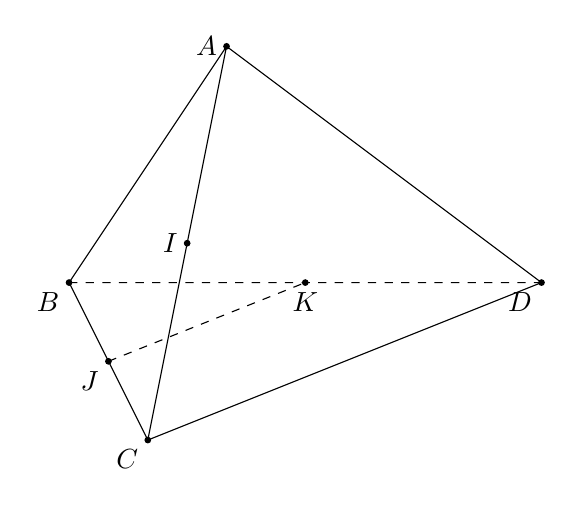
\begin{tikzpicture}
			\draw[fill=black] (0,0) circle (1pt) node[below left] {$B$};
			\draw[fill=black] (2,3) circle (1pt) node[ left] {$A$};
			\draw[fill=black] (6,0) circle (1pt) node[below left] {$D$};
			\draw[fill=black] (1,-2) circle (1pt) node[below left] {$C$};
			\draw[fill=black] (1.5,0.5) circle (1pt) node[left] {$I$};
			\draw[fill=black] (0.5,-1) circle (1pt) node[below left] {$J$};
			\draw[fill=black] (3,0) circle (1pt) node[below ] {$K$};
			\draw (0,0)--(1,-2)--(6,0) (0,0)--(2,3)--(1,-2) (2,3)--(6,0);
			\draw[dashed] (0,0)--(6,0) (0.5,-1)--(3,0);
	\end{tikzpicture}}
	\loigiai{
		Ta có $K \in(ABD) \cap(IJK)$
		mà $AB \parallel IJ$, $AB \subset (ABD)$; $IJ \subset (IJK)$.\\
		Suy ra $(ABD) \cap(IJK)=Kx \parallel AB \parallel IJ$.}
\end{ex}

%=======Câu 10
\begin{ex}%[1H4H5-3]
	Cho hình hộp $ABCD.A'B'C'D'$ có $AC$ cắt $BD$ tại $O$ còn $A'C'$ cắt $B'D'$ tại $O'$. Khi đó $\left(AB'D'\right)$ song song với mặt phẳng nào dưới đây?
	\choice
	{$\left(A'OC'\right)$}
	{$\left(BDA'\right)$}
	{$\left(BDC'\right)$}
	{$(BCD)$}
	
	\loigiai{
		\immini{	Vì $B'D' \parallel BD$ nên $B'D' \parallel\left(BDC'\right)$.\\
			Vì $AD' \parallel BC'$ nên $AD' \parallel\left(BDC'\right)$.\\
			Từ đó suy ra $\left(AB'D'\right) \parallel\left(BDC'\right)$.	}{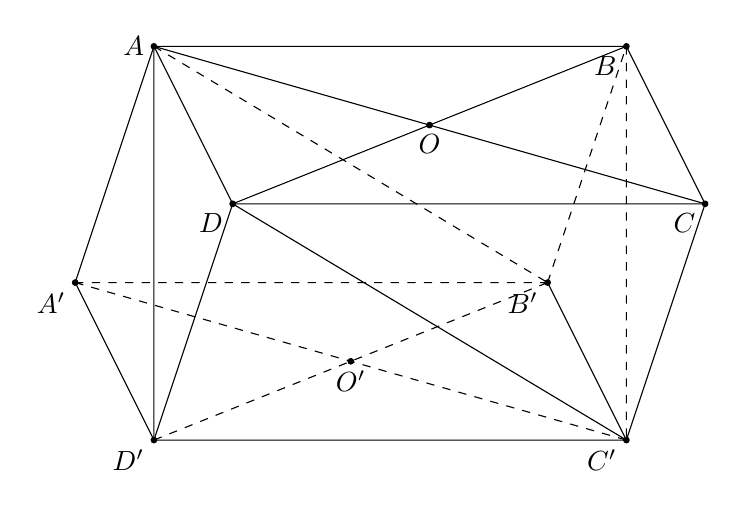
\begin{tikzpicture}
				\draw[fill=black] (0,0) circle (1pt) node[below left] {$A'$};
				\draw[fill=black] (1,3) circle (1pt) node[ left] {$A$};
				\draw[fill=black] (6,0) circle (1pt) node[below left] {$B'$};
				\draw[fill=black] (1,-2) circle (1pt) node[below left] {$D'$};
				\draw[fill=black] (7,-2) circle (1pt) node[below left] {$C'$};
				\draw[fill=black] (7,3) circle (1pt) node[below left] {$B$};
				\draw[fill=black] (2,1) circle (1pt) node[below left] {$D$};
				\draw[fill=black] (8,1) circle (1pt) node[below left] {$C$};
				\draw[fill=black] (4.5,2) circle (1pt) node[below] {$O$};
				\draw[fill=black] (3.5,-1) circle (1pt) node[below] {$O'$};
				\draw (0,0)--(1,-2)--(7,-2)--(6,0) (0,0)--(1,-2);
				\draw (1,3)--(7,3)--(8,1)--(2,1)--cycle;
				\draw[dashed] (0,0)--(6,0) (1,-2)--(6,0) (0,0)--(7,-2);
				\draw (0,0)--(1,3) (2,1)--(1,-2) (8,1)--(7,-2);
				\draw[dashed] (6,0)--(7,3) (1,3)--(6,0) (7,3)--(7,-2);
				\draw (8,1)-- (1,3) (7,3)--(2,1) (1,3)--(1,-2) (2,1)--(7,-2) ;
				
	\end{tikzpicture}}}
\end{ex}

%=======Câu 11
\begin{ex}%[1H4N6-2]
	Qua phép chiếu song song lên mặt phẳng $(P)$, hai đường thẳng chéo nhau $a$ và $b$ có hình chiếu là hai đường thẳng $a'$ và $b'$. Mệnh đề nào sau đây đúng?
	\choice
	{$a'$ và $b'$ luôn luôn cắt nhau}
	{$a'$ và $b'$ có thể trùng nhau}
	{$a'$ và $b'$ không thể song song}
	{$a'$ và $b'$ có thể cắt nhau hoặc song song với nhau}
	\loigiai{
		$a'$ và $b'$ có thể cắt nhau hoặc song song với nhau.}
\end{ex}

%=======Câu 12
\begin{ex}%[1D5N1-3]
	Điểu tra về chiều cao (đơn vị: cm ) của một số học sinh khối $11$, người ta có kết quả sau
	\begin{center}
		\begin{tabular}{|c|c|c|c|c|c|c|}
			\hline Chiều cao (cm) & {$[150 ; 154)$} & {$[154 ; 158)$} & {$[158 ; 162)$} & {$[162 ; 166)$} & {$[166 ; 170)$} & \\
			\hline Số học sinh & $8$ & $18$ & $40$ & $26$ & $8$ & $N=100$ \\
			\hline
		\end{tabular}
	\end{center}
	Chiều cao trung bình $(\mathrm{cm})$ của học sinh khối $11$ là
	\choice
	{$160{,}3$}
	{$161$}
	{\True $160{,}32$}
	{$160$}
	\loigiai{
		Ta có bảng giá trị đại diện nhóm
		\begin{center}
			\begin{tabular}{|c|c|c|c|c|c|c|}
				\hline Chiều cao (cm) & 152 & 156 & 160 & 164 & 168 & \\
				\hline Số học sinh & 8 & 18 & 40 & 26 & 8 & $N=100$ \\
				\hline
			\end{tabular}
		\end{center}
		Chiều cao trung bình là
		$$
		\overline{x}=\dfrac{152 \times 8+156 \times 18+160 \times 40+164 \times 26+168 \times 8}{100}=160{,}32.
		$$}
\end{ex}
\Closesolutionfile{ans}
% \indapan{7}{ans/11-CK1-Toan-tu-tam-De-2-Phan-1}
\cauds
\Opensolutionfile{ans}[ans/11-CK1-Toan-tu-tam-De-2-Phan-2]
\begin{ex}%[1D3H1-2]
	Biết giới hạn $\lim \dfrac{2n^2+1}{3n^3-3n+3}=a$ và $\lim \dfrac{n\sqrt{n^2+1}}{\sqrt{4n^4-n^2+3}}=b$. Khi đó
	\choiceTF
	{Giá trị $a$ nhỏ hơn $0$}
	{\True Giá trị $b$ lớn hơn $0$}
	{\True Phương trình lượng giác $\cos x=a$ có nghiệm là $x=\dfrac{\pi}{2}$}
	{Cho cấp số cộng $\left(u_n\right)$ với công sai $d=b$ và $u_1=a$ thì $u_3=\dfrac{3}{2}$}
	\loigiai
	{ \begin{itemchoice}
			\itemch Ta có $\lim \dfrac{2n^2+1}{3n^3-3n+3}=\lim \dfrac{n^3\left(\dfrac{2}{n}+\dfrac{1}{n^3}\right)}{n^3\left(3-\dfrac{3}{n^2}+\dfrac{3}{n^3}\right)}=\lim \dfrac{\dfrac{2}{n}+\dfrac{1}{n^3}}{3-\dfrac{3}{n^2}+\dfrac{3}{n^2}}=\dfrac{0}{3}=0$.\\
			Vậy $a=0$.
			\itemch  Ta có $\lim \dfrac{n\sqrt{n^2+1}}{
				\sqrt{4n^4-n^2+3}}=\lim \dfrac{n^2\sqrt{1+\dfrac{1}{n^2}}}{n^2\sqrt{4-\dfrac{1}{n^2}+\dfrac{3}{n^4}}}=\lim \dfrac{\sqrt{1+\dfrac{1}{n^2}}}{\sqrt{4-\dfrac{1}{n^2}+\dfrac{3}{n^4}}}=\dfrac{1}{2}$. \\
			Vậy $b=\dfrac{1}{2}$.
			\itemch Phương trình lượng giác $\cos x=0$ có một nghiệm là $x=\dfrac{\pi}{2}$. 			
			\itemch Cho cấp số cộng $\left(u_n\right)$với công sai $d=b=\dfrac{1}{2}$ và $u_1=a=0$ thì $u_3=0+2\cdot \dfrac{1}{2}=1$. 
		\end{itemchoice}
	}
	
\end{ex}
\begin{ex} %[1D3H2-7]
	Cho hàm số $f\left(x\right)=\heva{&x-2\ \text{khi}\ x<-1\\&\sqrt{x^2+1}+m \ \text{khi}\ x \geq -1.}$ Khi đó	
	\choiceTF
	{Giới hạn $\lim\limits_{x \to -2}f\left(x\right)=\sqrt{5}+m$ }
	{\True Giới hạn $\lim\limits_{x \to -1^-}f\left(x\right)=-3$  }
	{\True Giới hạn $\lim\limits_{x \to -1^+}f\left(x\right)=\sqrt{2}+m$ } 
	{Khi $m=3+\sqrt{2}$ thì hàm số đã cho có giới hạn tại $x_0=-1$ }
	\loigiai{
		\begin{itemchoice}
			\itemch Ta có $\lim\limits_{x \to -2}f\left(x\right)=-4$.
			
			\itemch  Xét dãy số $\left(x_n\right)$ bất kì sao cho $x_n<-1$ và $x_n \to -1$, ta có $f\left(x_n\right)=x_n-2$.\\
			Khi đó: $\lim \limits_{x\to -1^-}=\lim f\left(x_n\right)=-1-2=-3$. 
			\itemch Xét dãy số $\left(x_n\right)$ bất kì sao cho $x_n>-1$ và $x_n \to -1$, ta có $f\left(x_n\right)=\sqrt{x_n^2+1}+m$.\\ Khi đó $\lim\limits_{x \to -1^+}=\lim f\left(x_n\right)=\sqrt{\left(-1\right)^2+1}+m=\sqrt{2}+m$. 			
			\itemch Hàm số đã cho có giới hạn tại $x_0=-1$ khi\\ $\lim \limits_{x \to -1^-} f\left(x\right)=\lim \limits_{x \to -1^+} f\left(x\right)\Leftrightarrow m=-3-\sqrt{2}$.
		\end{itemchoice}
	}
\end{ex}
\begin{ex}%[1D3H3-3]
	Cho hàm số $f\left(x\right)=\heva{&\dfrac{4-x^2}{\sqrt{x+2}-2},x>2\\&mx+8,x\leq2.}$ ($m$ là tham số)
	\choiceTF
	{\True  Tập xác định của hàm số là $\mathscr{D}=\mathbb{R}$}
	{\True Hàm số liên tục tại $x=7$ với mọi $m$}
	{Hàm số không liên tục tại $x=0$ với mọi $m$}
	{\True Hàm số $f\left(x\right)$ liên tục tại điểm $x_0=2$ khi $m=-12$}
	\loigiai{
		\begin{itemchoice}
			\itemch Tập xác định của hàm số là $\mathscr{D}=\mathbb{R}$. 
			\itemch  Xét $f\left(x\right)=\dfrac{4-x^2}{\sqrt{x+2}-2},x>2$ \\ $f\left(7\right)=\dfrac{4-7^2}{\sqrt{7+2}-2}=-45$\\
			$\lim\limits_{x\to 7}f\left(x\right)=\lim\limits_{x\to 7}\dfrac{4-x^2}{\sqrt{x+2}-2}=\dfrac{4-7^2}{\sqrt{7+2}-2}=-45=f\left(7\right)$\\
			Suy ra hàm số liên tục tại $x=7$ với mọi $m$.
			\itemch Xét $f\left(x\right)=mx+8, x\leq 2$\\
			$f\left(0\right)=m\cdot 0+8=8$\\
			$\lim\limits_{x\to 0}f\left(x\right)=\lim\limits_{x\to 0}\left(mx+8\right)=2\cdot 0+8=8=f\left(2\right)$.\\
			Suy ra hàm số liên tục tại $x=0$ với mọi $m$. 			
			\itemch 
			\begin{eqnarray*}
				& &	\lim\limits_{x\to 2^+}\dfrac{4-x^2}{\sqrt{x+2}-2}\\
				&=&\lim \limits_{x \to 2^+}\dfrac{\left(4-x^2\right)\left(\sqrt{x+2}+2\right)}{x+2-4}\\
				&=& \lim \limits_{x \to 2^+}\dfrac{\left(2-x\right)\left(2+x\right)\left(\sqrt{x+2}+2\right)}{x-2}\\
				&=& \lim\limits_{x\to 2^+} \left[-2\left(2+x\right)\left(\sqrt{x+2}+2\right)\right]\\
				&=&-16
			\end{eqnarray*}
			$\lim\limits_{x \to 2^-}\left(mx+8\right)=2m+8=f\left(2\right)$.\\
			Để hàm số $f\left(x\right)$ liên tục tại $x_0=2$ thì\\ $\lim \limits_{x\to 2^+}f\left(x\right)=\lim \limits_{x\to 2^-}f\left(x\right)=f\left(2\right)\Leftrightarrow 2m+8=-16\Leftrightarrow m=-12	$.\\
			Vậy $m=-12$ thì hàm số $f\left(x\right)$ liên tục tại điểm $x_0=2$.
		\end{itemchoice}
	}
\end{ex}
\begin{ex}%[1H4V2-4]
	Cho hình chóp $S.ABCD$ có đáy là hình bình hành tâm $O$, $M$ là một điểm thuộc đoạn $SA$ sao cho $2MA=SM$, điểm $N$ là điểm thuộc tia đối của tia $OS$ sao cho $3ON=SO$, $G$ là trọng tâm tam giác $SCD$. Gọi $K=SD\cap \left(GMN\right)$.
	\choiceTF
	{\True $\dfrac{OE}{MA}=\dfrac{1}{2}$( từ $O$ dựng đường thẳng $d$ song song với $SA$, cắt $MN$ tại $E$)}
	{$\dfrac{AF}{AC}=\dfrac{2}{3}$ (gọi $F=MN\cap AC$) }
	{\True  $MN \parallel SC$}
	{\True $\dfrac{SK}{KD}=\dfrac{1}{2}$}
	\loigiai{
		\begin{center}
			
			\begin{tikzpicture}[declare function={gocx=80; goc=-150; a=4; b=a/2; h=3;}]
				\path (0,0) coordinate (A)--+(gocx:h) coordinate (S)
				(a,0) coordinate (D)
				(goc:b) coordinate (B)
				+(a,0) coordinate (C)
				($(A)!1/3!(S)$) coordinate (M)
				($(A)!1/2!(C)$) coordinate (O)
				($(A)!1/3!(S)$) coordinate (M)
				($(O)!-1/3!(S)$) coordinate (N)
				($(D)!1/2!(C)$) coordinate (T1)
				($(S)!1/2!(C)$) coordinate (I)
				(intersection of S--T1 and D--I) coordinate (G)
				(intersection of M--N and A--C) coordinate (F)
				;
				\draw[dashed] (S)--(A) (D)--(A)--(B) (A)--(C) (B)--(D) (S)--(N) (M)--(N)--(G)--(M);
				\draw (S)--(D)--(C)--(S)--(B)--(C)--cycle;
				\foreach \x/\goc in {S/90,A/150,B/-90,C/-60,D/0,O/50,N/-90,G/0,M/180,F/195,I/0}
				\draw[fill=white] (\x) node[shift={(\goc:7pt)},font=\scriptsize]{$\x$} circle (1pt);
			\end{tikzpicture}
			
		\end{center}
		\begin{itemchoice}
			\itemch Trong $\left(SAC\right)$, từ $O$ dựng đường thẳng $d$ song song với $SA$, cắt $MN$ tại $E$.\\ Ta có $OE \parallel SM\Rightarrow \dfrac{OE}{SM}=\dfrac{ON}{SN}=\dfrac{1}{4}\Rightarrow \dfrac{OE}{2MA}=\dfrac{1}{4}\Rightarrow \dfrac{OE}{MA}=\dfrac{1}{2}$.
			\itemch Gọi $F=MN \cap AC$. \\
			Trong $\left(SAC\right)$, gọi $F=MN\cap AC$ ta có \\$OE \parallel MA\Rightarrow \dfrac{OE}{MA}=\dfrac{OF}{AF}=\dfrac{1}{2}\Rightarrow \dfrac{AF}{AO}=\dfrac{2}{3}\Rightarrow \dfrac{AF}{AC}=\dfrac{1}{3}$.
			\itemch Ta có $\dfrac{AM}{SA}=\dfrac{AF}{AC}=\dfrac{1}{3}\Rightarrow MF \parallel SC\Rightarrow MN \parallel SC$. 			
			\itemch Ta có $\heva{&G \in \left(GMN\right)\cap \left(SCD\right)\\&MN \parallel SC\\&MN\subset \left(GMN\right),SC\subset \left(SCD\right) }\Rightarrow \heva{&xGx'=\left(GMN\right)\cap \left(SCD\right)\\&xGx' \parallel SC \left( \parallel MN\right).}$ \\
			Gọi $K=xGx'\cap SD\Rightarrow \heva{&K \in xGx',xGx'\subset \left(GMN\right)\\&K \in SD}\Rightarrow K=SD\cap \left(GMN\right)$.\\
			Ta có $GK\parallel SC\Rightarrow \dfrac{DK}{SD}=\dfrac{DG}{DI}=\dfrac{2}{3}$ ( với $I$ là trung điểm $SC$) $\Rightarrow \dfrac{SK}{KD}=\dfrac{1}{2}$.
		\end{itemchoice}
	}
\end{ex}


\Closesolutionfile{ans}
% \indapan{3}{ans/11-CK1-Toan-tu-tam-De-2-Phan-2}


\caukq
\Opensolutionfile{ans}[ans/ans-11-CK1-Toan-tu-tam-De-2-Phan-3-KQ]
%TLN-Cau-17
\begin{ex}%[1D2C3-6]
	Tam giác mà ba đỉnh của nó là ba trung điểm ba cạnh của tam giác $ABC$ được gọi là tam giác trung bình của tam giác $ABC$. Ta xây dựng dãy các tam giác $A_1B_1C_1$, $A_2B_2C_2$, $A_3B_3C_3$, $\ldots$ sao cho $A_1B_1C_1$ là một tam giác đều cạnh bằng $\sqrt{3}$ và với mỗi số nguyên dương $n \geq 2$, tam giác $A_nB_nC_n$ là tam giác trung bình của tam giác $A_{n-1}B_{n-1}C_{n-1}$. Với mỗi số nguyên dương $n$, kí hiệu $S_n$ tương ứng là diện tích hình tròn ngoại tiếp tam giác $A_nB_nC_n$. Tổng $S = S_1 + S_2 + S_3 + \cdots = a\pi$. Tìm $a$?
	
	\shortans{4}
	\loigiai
	{
		Vì dãy các tam giác $A_1B_1C_1$, $A_2B_2C_2$, $A_3B_3C_3$, $\ldots$ là các tam giác đều nên bán kính đường tròn ngoại tiếp các tam giác bằng cạnh $\times \dfrac{\sqrt{3}}{3}$.\\
		Với $n = 1$ thì tam giác đều $A_1B_1C_1$ có cạnh bằng $\sqrt{3}$ nên đường tròn ngoại tiếp tam giác $A_1B_1C_1$ có bán kính $R_1 = \sqrt{3} \times \dfrac{\sqrt{3}}{3} = 1 \Rightarrow S_1 = \pi \left( \sqrt{3} \times \dfrac{\sqrt{3}}{3} \right)^2$.\\
		Với $n = 2$ thì tam giác đều $A_2B_2C_2$ có cạnh bằng $\dfrac{\sqrt{3}}{2}$ nên đường tròn ngoại tiếp tam giác $A_2B_2C_2$ có bán kính $R_2 = \dfrac{\sqrt{3}}{2} \times \dfrac{\sqrt{3}}{3} = \dfrac{1}{2} \Rightarrow S_2 = \pi \left( \dfrac{\sqrt{3}}{2} \times \dfrac{\sqrt{3}}{3} \right)^2$.\\
		Với $n = 3$ thì tam giác đều $A_3B_3C_3$ có cạnh bằng $\dfrac{\sqrt{3}}{4}$ nên đường tròn ngoại tiếp tam giác $A_3B_3C_3$ có bán kính $R_3 = \dfrac{\sqrt{3}}{4} \times \dfrac{\sqrt{3}}{3} = \dfrac{1}{4} \Rightarrow S_3 = \pi \left( \dfrac{\sqrt{3}}{4} \times \dfrac{\sqrt{3}}{3} \right)^2$.\\
		Như vậy tam giác đều $A_nB_nC_n$ có cạnh bằng $\dfrac{\sqrt{3}}{2^{n-1}}$ nên đường tròn ngoại tiếp tam giác $A_nB_nC_n$ có bán kính $R_n = \dfrac{\sqrt{3}}{2^{n-1}} \times \dfrac{\sqrt{3}}{3} = \dfrac{1}{2^{n-1}} \Rightarrow S_n = \pi \left( \dfrac{\sqrt{3}}{2^{n-1}} \times \dfrac{\sqrt{3}}{3} \right)^2$.\\
		Khi đó ta được dãy $S_1$, $S_2$, $\ldots$, $S_n$, $\ldots$ là một cấp số nhân lùi vô hạn với số hạng đầu $u_1 = S_1 = \pi$và công bội $q = \dfrac{1}{4}$.\\
		Do đó tổng $S = S_1 + S_2 + S_3 + \cdots = \dfrac{u_1}{1 - q} = 4\pi$.\\
		Suy ra $a = 4$.
	}
\end{ex}
%TLN-Cau-18
\begin{ex}%[1D2C3-6]
	Cho hình vuông $\left( C_1 \right)$ có cạnh bằng $a$. Người ta chia mỗi cạnh của hình vuông thành bốn phần bằng nhau và nối các điểm chia một cách thích hợp để có hình vuông $\left( C_2 \right)$ (Hình vẽ).
	
	\begin{center}
		\begin{tikzpicture}[scale=0.7, font=\footnotesize, line join=round, line cap=round, >=stealth]
			
%			\draw[->] (-4,0)--(4,0) node[below left] {$x$};
%			\draw[->] (0,-4)--(0,4) node[below left] {$y$};
%			\draw (0,0) node [shift={(-130:3mm)}] {$O$};
			
			\path 
				(0,0) coordinate (A)
				(4,0) coordinate (B)
				(4,4) coordinate (C)
				(0,4) coordinate (D)
			;
			
			\draw (A) -- (B) -- (C) -- (D) -- cycle;
			\foreach \in in {1,...,10}{
				\path 
					($(A)!1/4!(B)$) coordinate (E)
					($(B)!1/4!(C)$) coordinate (F)
					($(C)!1/4!(D)$) coordinate (G)
					($(D)!1/4!(A)$) coordinate (H)
					
					(E) coordinate (A)
					(F) coordinate (B)
					(G) coordinate (C)
					(H) coordinate (D)
					
				;
				\draw (A) -- (B) -- (C) -- (D) -- cycle;
			}
			
		\end{tikzpicture}
	\end{center}
	
	Từ hình vuông $\left( C_2 \right)$ lại tiếp tục làm như trên ta nhận được dãy các hình vuông $C_1$, $C_2$, $C_3$, $\ldots$, $C_n$, $\ldots$. Gọi $S_i$ là diện tích hình vuông $C_i$ với $i \in \left\{1, 2, 3, \ldots \right\}$. Đặt $T = S_1 + S_2 + S_3 + \cdots + S_n + \cdots$ Tính độ dài $a$ biết $T = 4a + 12$?
	
	\shortans{3}
	\loigiai
	{
		Hình vuông $\left( C_1 \right)$ có cạnh bằng  $a$ và $S_1 = a^2$.\\
		Cạnh của hình vuông $\left( C_2 \right)$ là $a_2 = \sqrt{\left( \dfrac{3}{4}a \right)^2 + \left( \dfrac{1}{4}a \right)^2} = \dfrac{a\sqrt{10}}{4}$, \\
		diện tích $S_2 = a_2^2 = \dfrac{5}{8}a^2 = \dfrac{5}{8}S_1$.\\
		Cạnh của hình vuông $\left( C_3 \right)$ là $a_3 = \sqrt{\left( \dfrac{3}{4}a_2 \right)^2 + \left( \dfrac{1}{4}a_2 \right)^2} = \dfrac{a_2\sqrt{10}}{4} = a\left(\dfrac{\sqrt{10}}{4}\right)^2$,\\
		diện tích $S_3 = \left( \dfrac{5}{8}a \right)^2 = \dfrac{5}{8}S_2 = \left( \dfrac{5}{8} \right)^2 S_1$.\\
		Tương tự, diện tích của hình vuông $\left( C_i \right)$ là $S_i = \left( \dfrac{5}{8} \right)^{i-1} S_1 = \left( \dfrac{5}{8} \right)^{i-1} a^2$ và \\
		diện tích $S_n = \left( \dfrac{5}{8} \right)^{n-1} a^2$.\\
		Từ đó $T = S_1 + S_2 + S_3 + \cdots + S_n + \cdots = a^2 \left[ 1 + \dfrac{5}{8} + \left( \dfrac{5}{8} \right)^2 + \cdots + \left( \dfrac{5}{8} \right)^{n-1} + \cdots \right]$.\\
		Mà $P = 1 + \dfrac{5}{8} + \left( \dfrac{5}{8} \right)^2 + \cdots + \left( \dfrac{5}{8} \right)^{n-1} + \cdots$ là tổng của cấp số nhân lùi vô hạn với\\
		$u_1 = 1, q = \dfrac{5}{8} \Rightarrow P = \dfrac{1}{1 - \dfrac{5}{8}} = \dfrac{8}{3} \Rightarrow T = \dfrac{8}{3}a^2$.\\
		Suy ra $T = \dfrac{8}{3}a^2 = 4a + 12 \Leftrightarrow 8a^2 - 12a - 36 = 0 \Leftrightarrow \hoac{&a=3\\&a=-\dfrac{3}{2}.}$\\
		Vì $a > 0$ nên $a = 3$.
	}
\end{ex}
%TLN-Cau-19
\begin{ex}%[1D3C2-5]
	Cho biết $\lim\limits_{x \to +\infty} \left( \sqrt{x^2 + ax} + bx \right) = 2$, tính giá trị biểu thức $P = a + 2b$.
	
	\shortans{2}
	\loigiai
	{
		Do $\lim\limits_{x \to +\infty} \left( \sqrt{x^2 + ax}  + bx \right) = 2$ là một số hữu hạn, nên $b = -1$.\\
		Khi đó
		\begin{align*}
		\lim\limits_{x \to +\infty} \left( \sqrt{x^2 + ax }+ bx \right) 
		&= \lim\limits_{x \to +\infty} \left( \sqrt{x^2 + ax }- x \right)
		= \lim\limits_{x \to +\infty} \dfrac{ax}{\sqrt{x^2 + ax }+ x} \\
		&= \lim\limits_{x \to +\infty} \dfrac{ax}{x \left( \sqrt{1 + \dfrac{a}{x} }+ 1 \right)}
		= \dfrac{a}{2}.
		\end{align*}
		Theo giả thiết $\dfrac{a}{2} = 2 \Rightarrow a = 4$.\\
		Vậy $\heva{&a = 4 \\ &b = -1} \Rightarrow P = a + 2b = 2$.
	}
\end{ex}
%TLN-Cau-20
\begin{ex}%[1D3V3-4]
	Khi hàm số $f(x) = \heva{&\dfrac{x^2 + x - 2}{x - 1} && \text{ khi } x \neq 1 \\ &3m + 1 && \text{ khi } x = 1}$ liên tục trên $\mathbb{R}$, hãy tính giá trị biểu thức $P = 9m^2 + 6m - 2$.
	
	\shortans{6}
	\loigiai
	{
		Ta có hàm số $f(x) = \dfrac{x^2 + x - 2}{x - 1}$ liên tục trên các khoảng $(-\infty; 1)$ và $(1; +\infty)$.\\
		Tại $x = 1$:
		\begin{align*}
			&\lim_{x \to 1} f(x) = \lim_{x \to 1} \frac{x^2 + x - 2}{x - 1} = \lim_{x \to 1} (x + 2) = 3.\\
			&f(1) = 3m + 1.
		\end{align*}
		Hàm số liên tục trên $\mathbb{R}$ khi hàm số liên tục tại $x = 1$ khi và chỉ khi
		\begin{align*}
			&\lim\limits_{x \to 1} f(x) = f(1) \\
			\Leftrightarrow &\ 3 = 3m + 1\\
			\Leftrightarrow &\ m = \dfrac{2}{3}.
		\end{align*}
		Suy ra $P = 9m^2 + 6m - 2 = 9 \cdot \left( \dfrac{2}{3} \right)^2 + 6 \cdot \left( \dfrac{2}{3} \right) - 2 = 6$.
	}
\end{ex}
%TLN-Cau-21
\begin{ex}%[1H4V2-2]
	Cho hình chóp $S.ABC$ và một điểm $I$ nằm trong tam giác $ABC$. Các đường thẳng qua $I$ lần lượt song song với các đường thẳng $SA$, $SB$, $SC$ cắt các mặt phẳng $(SBC)$, $(SCA)$, $(SAB)$ tại $A'$, $B'$, $C'$. Tính $\dfrac{IA'}{SA} + \dfrac{IB'}{SB} + \dfrac{IC'}{SC}$.
	\begin{center}
		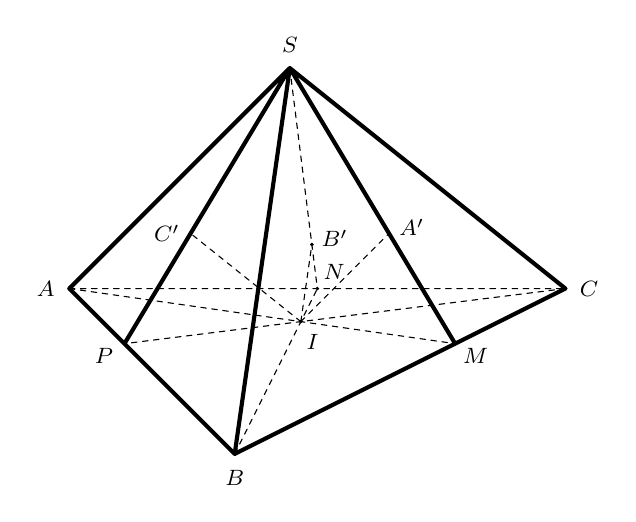
\begin{tikzpicture}[scale=0.7, font=\footnotesize, line join=round, line cap=round, >=stealth]
			\path 
				(0,0) coordinate (A)
				(3,-3) coordinate (B)
				(9,0) coordinate (C)
				(2.2,1) coordinate (C')
				(5.8,1) coordinate (A')
				(4.2,-0.6) coordinate (I)
				(4.4,0.8) coordinate (B')
				(7,-1) coordinate (M)
				(4.5,0) coordinate (N)
				(1,-1) coordinate (P)
				(4,4) coordinate (S)
			;
			
			\draw [line width=1.5pt]
				(A) -- (B) -- (C) -- (S) -- (A)
				(S) -- (P)
				(S) -- (M)
				(S) -- (B)
			;
			
			\draw[dash pattern=on 2pt off 2pt] 
				(A) -- (C)
				(S) -- (N)
				(A) -- (M)
				(B) -- (N)
				(C) -- (P)
				(I) -- (A')
				(I) -- (B')
				(I) -- (C')
			;
			\foreach \d/\v in {A/180, B/-90, C/0, S/90, M/-30, N/45, P/-150, I/-60, A'/15, B'/15, C'/180}{
				\fill[black] (\d) circle(1pt) node[shift={(\v:3mm)}] {$\d$};
			};
			
		\end{tikzpicture}
	\end{center}
	\shortans{1}
	\loigiai
	{
		Trong mặt phẳng $(ABC)$, gọi $M$ là giao điểm của $AI$ và $BC$.\\
		Trong mặt phẳng $(SAM)$, kẻ $IA'$ song song $SA$ cắt $SM$ tại $A'$.\\
		Điểm $A'$ là điểm cần tìm. Tương tự ta xác định các điểm $B'$, $C'$.\\
		Ta có $\dfrac{IA'}{SA} = \dfrac{MI}{MA}$.\\
		Mà $\dfrac{S_{IBC}}{S_{ABC}} =  \dfrac{\dfrac{1}{2}\mathrm{d}(I, BC) \cdot BC}{\dfrac{1}{2} \mathrm{d}(A, BC) \cdot BC} = \dfrac{\mathrm{d}(I, BC)}{\mathrm{d}(A, BC)} = \dfrac{MI}{MA}$.\\
		Nên $\dfrac{S_{IBC}}{S_{ABC}} = \dfrac{IA'}{SA}$.\\	
		Tương tự ta có $\dfrac{S_{IAC}}{S_{ABC}} = \dfrac{IB'}{SB}$ và $\dfrac{S_{IAB}}{S_{ABC}} = \dfrac{IC'}{SC}$.\\
		Suy ra $\dfrac{IA'}{SA} + \dfrac{IB'}{SB} + \dfrac{IC'}{SC} = \dfrac{S_{IBC}}{S_{ABC}} + \dfrac{S_{IAC}}{S_{ABC}} + \dfrac{S_{IAB}}{S_{ABC}} = \dfrac{S_{IBC} + S_{IAC} + S_{IAB}}{S_{ABC}} = \dfrac{S_{ABC}}{S_{ABC}} = 1$.\\
		Vậy $\dfrac{IA'}{SA} + \dfrac{IB'}{SB} + \dfrac{IC'}{SC} = 1$.
	}
\end{ex}
%TLN-Cau-22
\begin{ex}%[1H4C3-4]
	Cho hình chóp $S.ABCD$ có đáy là hình bình hành. Trên cạnh $SC$ lấy điểm $M$ sao cho $SM = \dfrac{1}{2} SC$. Mặt phẳng $(P)$ chứa $AM$ và song song với $BD$. Gọi $E$, $F$ lần lượt là giao điểm của $(P)$ với các cạnh $SB$, $SD$. Tính tỉ số $\dfrac{SE}{SB} + \dfrac{SF}{SD}$. \textit{(Kết quả làm tròn đến hàng phần mười)}.
	\begin{center}
		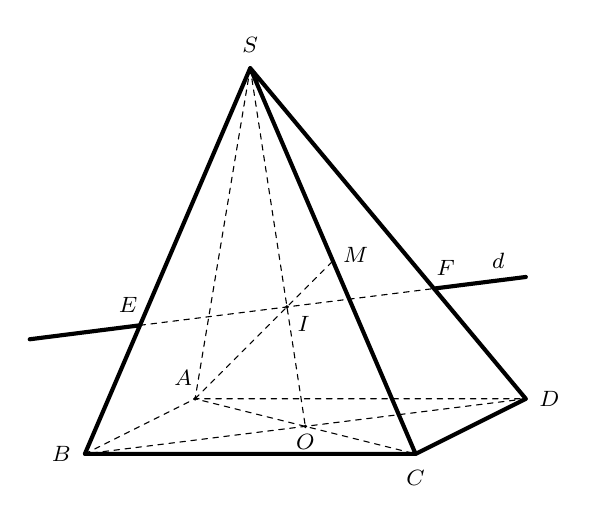
\begin{tikzpicture}[scale=0.7, font=\footnotesize, line join=round, line cap=round, >=stealth]
			
			\path 
				(2,1) coordinate (A)
				(0,0) coordinate (B)
				(6,0) coordinate (C)
				(8,1) coordinate (D)
				(1,7/3) coordinate (E)
				(19/3,3) coordinate (F)
				(-1,0) coordinate (H)
				(11/3,8/3) coordinate (I)
				(8,0) coordinate (J)
				(4.5,3.5) coordinate (M)
				(4,0.5) coordinate (O)
				(3,7) coordinate (S)
				(-1,2.08) coordinate (d_1)
				(8,3.21) coordinate (d_2)
			;
			
			\draw[dash pattern=on 2pt off 2pt] 
				(B) -- (A) -- (D) -- (B)
				(S) -- (A) -- (C)
				(S) -- (O)
				(E) -- (F)
				(A) -- (M)
			;
			\draw[line width=1.5pt] 
				(S) -- (B) -- (C) -- (D) -- (S)
				(S) -- (C)
				(d_2) -- (F)
				(d_1) -- (E)
			;
			
			\foreach \i/\j in {A/120, B/180, C/-90, D/0, S/90, E/120, F/60, M/15, I/-45}{
				\fill[black] (\i) circle(1pt) node[shift={(\j:3mm)}] {$\i$};
			}
			\fill[black] (O) circle(1pt) node[shift={(-90:2mm)}]{$O$};
			\draw (d_2) +(180:5mm) node[shift={(90:2mm)}] {$d$};
		\end{tikzpicture}
	\end{center}
	
	\shortans{1{,}3}
	\loigiai
	{
		Gọi $O$ là giao điểm của $AC$ và $BD$.\\		
		Ta có $\heva{&AM \cap SO = \{ I \}\\&AM \subset (P)\\&SO \subset (SBD)} \Rightarrow I \in (P) \cap (SBD)$.\\
		Mà $(SBD) \supset SD \parallel (P)$, suy ra $(P) \cap (SBD) = d \parallel BD$ với $I \in d$.\\
		Gọi $E = d \cap SB$, $F = d \cap SD$.\\
		Khi đó $E$, $F$ chính là là giao điểm của $(P)$ với các cạnh $SB$, $SD$.\\
		Xét tam giác $SAC$, có $O$ là trung điểm của $AC$, $M$ là trung điểm của $SC$ $\left( SM = \dfrac{1}{2} SC \right)$.\\
		$\Rightarrow I$ là trọng tâm của tam giác  $SAC \Rightarrow \dfrac{SI}{SO} = \dfrac{2}{3}$.\\
		Mặt khác $EF \parallel BD$, suy ra:\\
		$\dfrac{SE}{SB} = \dfrac{SF}{SD} = \dfrac{SI}{SO} = \dfrac{2}{3}$.\\
		$\Rightarrow \dfrac{SE}{SB} + \dfrac{SF}{SD} = \dfrac{2}{3} + \dfrac{2}{3} = \dfrac{4}{3} \approx 1{,}3$.
	}
\end{ex}

\Closesolutionfile{ans}
% \indapan{6}{ans/ans-11-CK1-Toan-tu-tam-De-2-Phan-3-KQ}